\documentclass[a4paper,12pt]{report}

\usepackage[utf8]{inputenc}
\usepackage[french]{babel}
\usepackage[T1]{fontenc}
\usepackage[scaled]{helvet} % police
\usepackage{lmodern}
\usepackage{layout}
\usepackage[top=2cm, bottom=2cm, left=3cm, right=2cm]{geometry}
\usepackage{setspace}
\usepackage{verbatim}
\usepackage{moreverb}
\usepackage{listings}
\usepackage{graphicx}
\usepackage{shorttoc}
\usepackage{glossaries}
\usepackage{xcolor}

\usepackage{xcolor}
%\usepackage{biblatex} 

% Tête de chapitre
\makeatletter
\newlength{\chapter@number@width}
\def\@makechapterhead#1{%
  {\normalfont
  \setlength{\parindent}{0pt}%
  \vspace*{10pt}%
  \settowidth{\chapter@number@width}{%
    \hbox{\color{white}\LARGE\bfseries
          \hspace{\dimexpr 1mm+3pt}%
          \thechapter
          \hspace{\dimexpr 1mm+3pt}%
    }}
  \hbox{%
    \vtop{%
      \hsize=\dimexpr\chapter@number@width+\tabcolsep+2\fboxrule+\tabcolsep
      \begin{tabular}[t]{@{}c}
        \scshape\strut\makebox[0pt]{\hspace{0pt plus 1 fill minus 1 fill}\@chapapp\hspace{0pt plus 1 fill minus 1 fill}} \\
        \fboxsep=0pt
        \colorbox{black}{\vbox{%
           \hbox{\vbox to \dimexpr 1mm+3pt{}}
           \hbox{\color{white}\LARGE\bfseries
                 \hspace{\dimexpr 1mm+3pt}%
                 \thechapter
                 \hspace{\dimexpr 1mm+3pt}%
                }
           \hrule height 0.4pt depth 0pt width 0pt
           \hbox{\vbox to 6pt{}}
           \hbox{\parbox{0pt}{\Huge\bfseries\vphantom{E}}}
           }}%
      \end{tabular}%
      }%
    \vtop{%
      \advance\hsize by -\dimexpr\chapter@number@width+2\fboxrule+\tabcolsep
      \hspace*{-0.5cm}\begin{tabular}[t]{c}
        \scshape\strut\vphantom{\@chapapp} \\
        \fboxsep=0pt
        \colorbox{white}{\vbox{%
           \hbox{\vbox to \dimexpr 1mm+3pt{}}
           \hbox{\LARGE\bfseries
                 \hspace{\dimexpr 1mm+3pt}%
                 \phantom{\thechapter}
                 \hspace{\dimexpr 1mm+3pt}%
                }
           \hrule height 0.4pt depth 0pt width \hsize
           \hbox{\vbox to 6pt{}}
           \hbox{\hspace*{20pt}\parbox{\dimexpr\textwidth-2mm-6pt-\chapter@number@width-\tabcolsep-2\fboxrule-20pt}{\Huge\bfseries #1}}
           }}%
      \end{tabular}%
      }%
    }%
  \vspace{50pt}%
  }
}
\def\@makeschapterhead#1{%
  {\normalfont
  \setlength{\parindent}{0pt}%
  \vspace*{10pt}%
  \settowidth{\chapter@number@width}{%
    \hbox{\color{white}\LARGE\bfseries
          \hspace{\dimexpr 1mm+3pt}%
          \thechapter
          \hspace{\dimexpr 1mm+3pt}%
    }}
  \hbox{%
    \vtop{%
      \hsize=\dimexpr\chapter@number@width+\tabcolsep+2\fboxrule+\tabcolsep
      \begin{tabular}[t]{@{}c}
        \scshape\strut\makebox[0pt]{\hspace{0pt plus 1 fill minus 1 fill}\phantom{\@chapapp}\hspace{0pt plus 1 fill minus 1 fill}} \\
        \fboxsep=0pt
        \colorbox{black}{\vbox{%
           \hbox{\vbox to \dimexpr 1mm+3pt{}}
           \hbox{\color{white}\LARGE\bfseries
                 \hspace{\dimexpr 1mm+3pt}%
                 \phantom{\thechapter}%
                 \hspace{\dimexpr 1mm+3pt}%
                }
           \hrule height 0.4pt depth 0pt width 0pt
           \hbox{\vbox to 6pt{}}
           \hbox{\parbox{0pt}{\Huge\bfseries\vphantom{E}}}
           }}%
      \end{tabular}%
      }%
    \vtop{%
      \advance\hsize by -\dimexpr\chapter@number@width+2\fboxrule+\tabcolsep
      \hspace*{-0.5cm}\begin{tabular}[t]{c}
        \scshape\strut\vphantom{\@chapapp} \\
        \fboxsep=0pt
        \colorbox{white}{\vbox{%
           \hbox{\vbox to \dimexpr 1mm+3pt{}}
           \hbox{\LARGE\bfseries
                 \hspace{\dimexpr 1mm+3pt}%
                 \phantom{\thechapter}
                 \hspace{\dimexpr 1mm+3pt}%
                }
           \hrule height 0.4pt depth 0pt width \hsize
           \hbox{\vbox to 6pt{}}
           \hbox{\hspace*{20pt}\parbox{\dimexpr\textwidth-2mm-6pt-\chapter@number@width-\tabcolsep-2\fboxrule-20pt}{\Huge\bfseries #1}}
           }}%
      \end{tabular}%
      }%
    }%
  \vspace{50pt}%
  }
}
\makeatother

% Redéfinition de commandes
\renewcommand\thesection{\arabic{section}}
% \renewcommand\thechapter{\Roman{chapter}}
\renewcommand*\familydefault{\sfdefault} %% Only if the base font of the document is to be sans serif

\makeglossaries
\newglossaryentry{ASP}{
	name={ASP}, % apparait dans le glossaire
	text={ASP*}, % apparait dans le texte
	description={Application Service Provider,  Fournisseur d'Applications de Service}
}

\title{Le cloud et la virtualisation}
\author{Sébastien Corbin et Gaëlle Avrillon}
\date{\today}


\begin{document}
% Interlignage 1,5
\begin{onehalfspace}

		\begin{titlepage}
			\begin{center}
				Sébastien CORBIN et Gaëlle AVRILLON\\
				CSII 3\ieme année\\
			\end{center}
			\hrulefill
			\vspace{7cm}
			\begin{center} 
				\LARGE \textbf{La virtualisation et le cloud}\\
			\end{center}
		\end{titlepage}
		\newpage

		\shorttableofcontents{Sommaire}{0}
		\setcounter{page}{1}
		\thispagestyle{empty}
		\newpage

	%%%%%%%%%%%%%%%%%%
	% Introduction 
	%%%%%%%%%%%%%%%%%%
	\chapter*{Introduction}
	
	\paragraph*{}
	Le Cloud Computing est un concept qui consiste à déporter sur des serveurs distants des traitements informatiques (applications, données) traditionnellement localisés sur des serveurs locaux ou encore sur le poste client de l’utilisateur. En français, l’anglicisme “Cloud Computing” est largement utilisé. Cependant, on rencontre de nombreuses traductions telles que “informatique dans les nuages”, “informatique dématérialisée”, “informatique virtuelle”, ou encore “infonuagique”.

	\paragraph*{}
	Les utilisateurs ou les entreprises ne gèrent plus leurs serveurs informatiques mais peuvent accéder de manière évolutive à de nombreux services en ligne. Les applications et les données de sont plus présentes sur l’ordinateur local mais dans le nuage (“Cloud”). Le Cloud est composé d’un certains nombre de serveurs interconnectés. L’accès à ses services s’effectue la plupart du temps à l’aide d’un navigateur web.
	
	\paragraph*{}
	Le concept d'informatique dans le nuage est comparable à celui de la distribution de l'énergie électrique. La puissance de calcul et de stockage de l'information est proposée à la consommation par des entreprises spécialisées et facturé d'après l'utilisation réelle. Ainsi, les entreprises n'ont plus besoin de serveurs dédiés, mais confient cette ressource à une entreprise qui leur garantit une puissance de calcul et de stockage à la demande.
	
	\paragraph*{}
	Le Cloud a émergé pour répondre aux exigences de continuité de qualité de service. Le Cloud est la mise en flexibilité de 4 niveaux : l’application (en contact avec le client), la plateforme (qui exécute les applications), l’infrastructure (qui est le support de la plateforme) et les données (qui sont fournies sur demande).
	
	\paragraph*{}
	Plus de 100 milliards d’euros (selon CloudHyperMarket) ont été investi dans le cloud computing. Les deux principaux acteurs du Cloud Computing sont Microsoft et Google. Microsoft a investi 9.6 milliard de dollars en 2011 dans le cloud soit 90\% de ses dépenses en recherche et développement. 4 millions d’entreprises ont fait confiance à Google et sont passées à Google Apps. Elles profitent à présent de grandes améliorations en termes de collaboration et d'économies.
	
	\paragraph*{}
	On trouve les premières traces du “cloud computing” dans les années 1960, quand Johan McCarty affirmait que cette puissance de traitement informatique serait accessible au public dans le futur. On parlait alors de Bureaux de Services (Service bureaus). C’est l’ancêtre du Software as a Service. Leur point commun est qu’ils offrent un service en échange d’honoraires. Leur application dans les domaines est vaste : banques, assurances, etc. Une entreprise de ce type offre à ses clients son expertise dans un domaine : cela correspond tout à fait avec la notion actuelle de Software As A Service (SaaS) et c’est par l’avancée technologique des réseaux de communications que cette notion de “bureaux de service”  s’est énormément développée dans l’informatique.
	
	\paragraph*{}
	Cependant, les débuts du cloud computing se situent dans la notion de Fournisseur de Service d’Application (ou en anglais Application Service Provider, ASP), présente au début des années 2000. Les premières applications à avoir migré dans les nuages sont les messageries, les outils collaboratifs, le CRM*, les environnements de développement. Amazon, Yahoo et Google sont les premiers à se lancer dans ce concept. Ces deux derniers offrent au grand public des applications simples et gratuites telles que la messagerie ou la gestion de calendriers en ligne.
	
	\paragraph*{}
	Le Grid Computing est une infrastructure virtuelle constituée d’un ensemble de ressources informatiques. Ces ressources sont partagées (elles sont mises à disposition des consommateurs), distribuées (elles sont situées dans des lieux géographiques différents), hétérogènes, coordonnées, autonomes et délocalisées (les ressources peuvent appartenir à plusieurs sites). On parle de “fermes de serveurs” (computer cluster en anglais) pour désigner cette technique qui consiste à regrouper plusieurs ordinateurs / serveurs indépendants. Cette technique permet une gestion globale, augmente la disponibilité des ressources, facilite la montée en charge et permet une répartition des charges entre les différents serveurs.
	Une des premières entreprises à avoir utilisé cette technique est Google, celui-ci a du créer des fermes de serveurs spécialisées pour répondre au nombre gigantesque de requêtes devant être traitées chaque seconde.
	
	\paragraph*{}
	Le terme Software as a Service (abrégé SaaS) est apparu en 2007 et remplace les précédents termes tels que ASP (Application Service Provider) ou encore “On Demand”.
	C’est un concept consistant à proposer un abonnement au logiciel plutôt que l’achat d’une licence. Avec le développement des technologies de l’information, de nombreuses offres SaaS se font à travers le web. Il n’y a alors plus besoin d’installer d’application de bureau, mais d’utiliser un programme client-serveur.
	Les applications s’appuyant sur ce modèle ont été nativement conçues pour le web contrairement aux modèles précédents.
	
	\paragraph*{}
	La crise de 2008-2009 a fait de gros dégâts dans la plupart des secteurs d’activités. La principale préoccupation des gérants d’entreprise est d’économiser afin de limiter les effets de la crise sur leur structure. Le service informatique est un service qui coûte cher. En effet, il faut prendre en compte les salaires, les assurances, les locaux, le matériel informatique, ... Ces dépenses peuvent être réduites voire totalement éliminées grâce au cloud computing. Le cloud computing permet de s'affranchir des coûts d'installation et de maintenance du matériel informatique et des logiciels en interne, on peut également s'affranchir des employés effectuant cette tâche, et par conséquent de leur salaire, de leur matériel et de leurs locaux. Une économie non négligeable à l'échelle d'une petite comme d'une grande entreprise.

	Mais les gains en termes de coût ne sont pas la seule raison qui peuvent pousser les entreprises à choisir le cloud computing. Devant les besoins d'évolutivité et de flexibilité des grands acteurs de l'informatique, les notions comme le Grid Computing ou la virtualisation sont devenues incontournables.
	
	% TODO : faire un renvoi vers le grid computing
	
	\paragraph*{}
	Nous étudierons dans ce rapport \textbf{l’apport des technologies du Cloud dans les entreprises}.
	
	\paragraph*{}
	En effet, le Grid Computing trouve ses bases dans la virtualisation (voir ci-dessus), celle-ci étant même le fondement du Cloud. Elle permet entre autres de faire fonctionner plusieurs systèmes d’exploitation sur un serveur physique au lieu d’en installer un par machine physique. Un autre objectif de la virtualisation est de pouvoir tester des applications sur des serveurs virtuels au lieu de serveurs physiques sans risques.
	
	Ces serveurs peuvent être hébergés au sein d’une entreprise ou chez un fournisseur de Cloud. Ainsi, on distingue trois architectures du Cloud : les clouds privés, les clouds publiques et les clouds hybrides. Le cloud privé est géré en interne par une entreprise pour ses propres besoins. Le cloud publique est géré par des entreprises spécialisées (les fournisseurs de services). Ces fournisseurs vont louer des ressources et des services à des entreprises ou à des particuliers. Enfin, le cloud hybride correspond à l’utilisation de plusieurs clouds (privés ou publiques).
	
	\paragraph*{}
	Dans un premier temps, nous présenterons le Cloud Computing. Puis, nous nous placerons dans un contexte d’entreprise afin d’étudier les besoins en terme de sécurité, de rentabilité et de flexibilité. Nous établirons également un cahier des charges type. Nous détaillerons ensuite les solutions techniques : les différentes architectures, la virtualisation. Nous finirons par un cas pratique en entreprise.
	
	
	
	%%%%%%%%%%%%%%%%%%%%%%%%%%
	\chapter{Présentation du Cloud Computing}
	%%%%%%%%%%%%%%%%%%%%%%%%%%


	%%%%%%%%%%%%%%%%%%%%%%%%%%
	\section{Définition du Cloud Computing}
	
	Le “Cloud Computing” est un néologisme utilisé pour décrire l’association d’Internet (“cloud”, le nuage) et l’utilisation de l’informatique (“computing”). On utilise l’informatique de manière dynamique et évolutive. Toutes les ressources sont fournies sous la forme de services à travers Internet. Les utilisateurs n’ont besoin d’aucune connaissance technique des services proposés.

	\paragraph*{}
	Ce concept inclut les infrastructures en tant que service (Infrastructure as a Service ou IaaS), les plateformes en tant que service (Platform as a Service ou PaaS), les applications en tant que service (Software as a Service ou SaaS) ainsi que le “Web 2.0” (aspect social d’Internet) et toutes les technologies récentes. Ces technologies dépendent presque exclusivement d’Internet pour répondre aux besoins des utilisateurs. Des exemples de fournisseurs de SaaS sont Salesforce.com ou encore Google Apps. Ils fournissent des outils professionnels accessibles par un navigateur web. Les applicatifs et les données sont stockés sur des serveurs distants.
	
	\paragraph*{}
	Le “cloud computing” correspond donc au développement et à l’utilisation d’applications accessibles uniquement par Internet. L’utilisateur a juste besoin d’Internet pour utiliser les applications, il n’a pas besoin d’installer un quelconque logiciel sur son poste. Les informations sont stockées de façon permanente sur Internet.
	
	\paragraph*{}
	La démocratisation des connexions Internet “haut débit” ainsi que l'accroissement de la capacité et de la puissance des disques durs et des processeurs ont permis le développement du “cloud computing”. Les utilisateurs louent du matériel auprès de leurs fournisseurs de service qui peuvent servir des millions de clients avec seulement des centaines de serveurs.
	
	\paragraph*{}
	Le cloud computing est perçu aujourd'hui comme quelque chose d'extrêmement puissant, capable de résoudre plusieurs milliards de milliards (1018) de traitements informatiques à la seconde, ce qui est largement supérieur à n'importe lequel des ordinateurs de bureau modernes seulement capables de milliers de milliards (1012) d'opérations à la seconde.
	
	\paragraph*{}
	Cette puissance est fournie par des architectures distribuées constituées d'ordinateurs « low-cost » (peu coûteux) qui s'échangent et se distribuent le travail en permanence. Elle est désormais à disposition de n'importe qui au travers d'Internet, que ce soit pour des utilisations financières (analyses), scientifiques (climat, statistiques) ou même médicales.
	

	%%%%%%%%%%%%%%%%%%%%%%%%%%
	\section{Les briques du Cloud Computing}

	Le cloud computing est une évolution naturelle des concepts de virtualisation, d’architecture basée sur les services (SaaS), et d’Utility Computing. Les utilisateurs n’ont plus besoin de détenir l’expertise du domaine informatique, ils louent la totalité de leur système d’information.

	\paragraph*{}
	Le schéma du cloud computing peut se résumer en :
	
	\begin{center}
		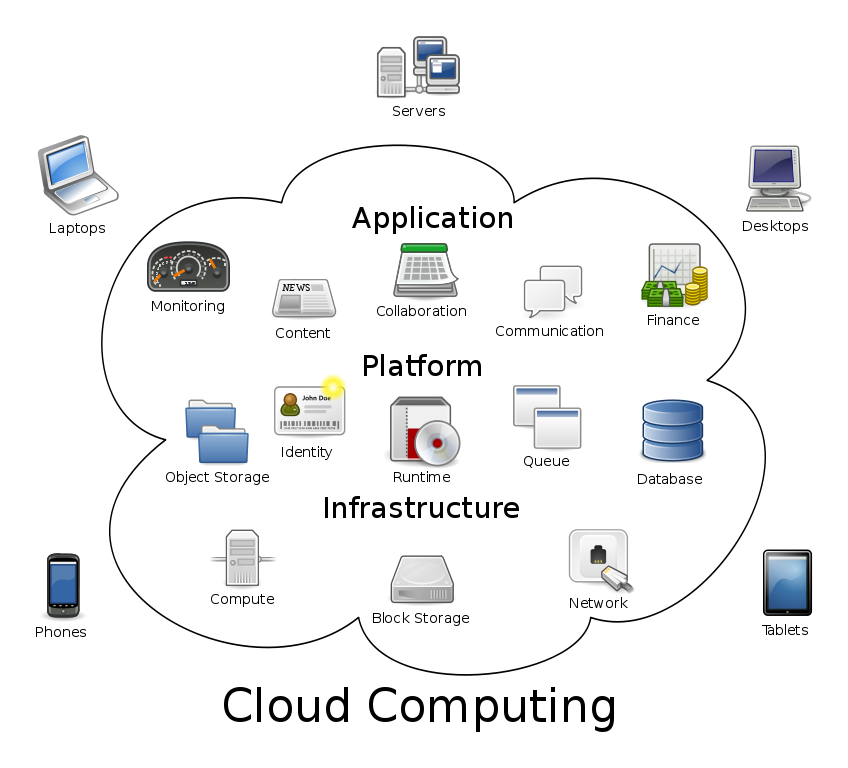
\includegraphics[width=15cm]{schema_structure.png}
	\end{center}
	
	On distingue ainsi 3 briques principales dans le Cloud :
	\begin{itemize}
		\item Application (Software as a service, SaaS)
		\item Platform (Platform as a service, PaaS)
		\item Infrastructure (Infrastructure as service, IaaS)
	\end{itemize}
	
	\subsection{Application (SaaS)}
	L’acronyme “SaaS” est le plus connu dans le monde du cloud computing. Sa signification est “Software as a Service”, autrement dit “application en tant que service”.
	
	Les différents services loués par le fournisseur sont disponibles sur le web, accessibles via un navigateur et vont de la messagerie à l’ERP en passant par des outils collaboratifs (documents, agenda, etc.) ou la comptabilité en ligne. Cette méthode supprime la nécessité d’installer une application sur le poste client et permet de diminuer les coûts du parc informatique interne à l’entreprise cliente, simplifiant par la même le support et la maintenance du service.
	
	\paragraph*{}
	\underline{Exemples :}
	\begin{itemize}
		\item CRM Salesforce.com (http://www.salesforce.com)
		\item Google Docs (http://docs.google.com)
		\item Adobe Photoshop Express Online (http://www.photoshop.com/express)
	\end{itemize}

	\subsection{Application (SaaS)}
	Le “PaaS” (“Platform as a Service” ou encore plate-forme en tant que service) a pour rôle l’exécution du logiciel. Elle est composée de briques utilisant des langages de programmation de haut niveau, généralement des langages de script (console de commande, Python, SQL, serveur d'application, etc.). La fonction logicielle doit être assurée correctement et continuellement. On utilise pour cela des “nuages” de serveurs. Les techniques utilisées sont variées : le basculement (fail-over) ou la répartition des charges (load-balancing). Le basculement est la capacité d’un équipement à basculer automatiquement vers un chemin réseau alternatif ou en mode veille. La répartition des charges est une technique permettant de distribuer un travail entre différents processus, ordinateurs, disques. C'est une architecture sans téléchargement ou installation de logiciels pour les développeurs, responsables informatiques ou utilisateurs finaux. Elle est également connue sous le nom de « cloudware ». Le PaaS offre des services tels que le travail collaboratif, l’intégration de web services et des bases de données ou encore la gestion de la sécurité, de la capacité, de la persistance des données ou le contrôle des versions.
	
	Ces services sont fournis au travers d’une solution complète destinée aux développeurs et disponible via Internet.
	
	\paragraph*{}
	\underline{Exemples :}
	\begin{itemize}
		\item Force.com (http://www.salesforce.com/platform)
		\item Google App Engine (http://appengine.google.com)
		\item Azure Services Platform (http://www.microsoft.com/azure)
	\end{itemize}
	
	\subsection{Infrastructure (IaaS)}
	L’”Infrastructure as a Service” (IaaS) gère les fonctionnalités de plus bas niveau, telles que le stockage et le réseau. Ce terme était originellement connu sous le nom de « Hardware as a Service ». C’est elle qui fait la liaison entre les différents datacenters du fournisseur pour que la disponibilité des informations soit continue et la gestion invisible pour l’utilisateur.
	
	Cette partie inclut également les ressources disponibles pour fournir le service, soit le volume de stockage et la capacité de calcul, très importante dans le Cloud Gaming (jeux en ligne dont les graphismes sont gérés côté serveur). La réplication ou la sauvegarde des données est également faite à ce niveau.
	
	Au lieu d’acheter des serveurs, des logiciels, des équipements réseau, les clients louent ces ressources auprès de leurs fournisseurs de service complètement externalisés et directement compétents dans le domaine.
	
	Le service est alors tarifé en fonction de l'utilisation et de la quantité de ressources consommées. De ce fait, le coût reflète le niveau d'activité de chaque client. C'est une évolution de l'hébergement Internet qui se différencie des anciens modes de fonctionnement :
	
	\begin{description}
		\item[Hébergement mutualisé] : une machine pour plusieurs clients, gérée par un prestataire de service et dont les clients payent le même prix peu importe leur utilisation.
		\item[Hébergement dédié] : une machine par client, gérée le plus souvent par le client lui même et pour laquelle le client paye le même prix chaque mois peu importe son utilisation.
		\item[Infrastructure as a Service] : un nombre indéfini de machines pour un nombre indéfini de clients, dont les ressources sont combinées et partagées pour tous les clients. Chaque client paye en fonction de son utilisation de l'architecture.
	\end{description}
	
	\paragraph*{}
	\underline{Exemples :}
	\begin{itemize}
		\item Amazon EC2 (http://aws.amazon.com)
		\item GoGrid (http://www.gogrid.com)
		\item Sun Grid (http://www.sun.com/software/sge)
	\end{itemize}
	
	%%%%%%%%%%%%%%%%%%%%%%%%%%
	\section{Les avantages du Cloud}
	
	Les avantages du Cloud Computing sont nombreux aussi bien du côté du fournisseur que du côté du client.
	
	\subsection{Les avantages du côté fournisseur}
	
	\paragraph*{}
	Tout d’abord, à cause de la crise économique, les entreprises cherchent à réduire les coûts et d’augmenter les marges. Le domaine du “cloud computing” permet de réaliser des économies d’échelle en se tournant vers le “cloud computing”.

	\paragraph*{}
	Ensuite, le cloud computing permet de surfer sur la vague du “web 2.0”. Le web 2.0 désigne les technologies et les usages du World Wide Web qui ont suivi la forme initiale du web, en particulier les interfaces permettant aux internautes d'interagir simplement à la fois avec le contenu des pages mais aussi entre eux, créant ainsi le web social. Le “web 2.0” est “à la mode” avec notamment les réseaux sociaux. Par exemple, le réseau social Facebook doit supporter 100 siècles de temps de connexion cumulés par jour et des milliards de contenus sont partagés sur la plateforme chaque jour. En 2010, Youtube a du prendre en charge l’hébergement de 24 heures de vidéos par minute.

	Que serait ces sites sans l’apport de solutions et d’infrastructures ultra-flexibles et facilement maintenables telles que le cloud computing peut supporter ? Le Web 2.0 a révolutionné l’Internet d’aujourd’hui au prix d’une demande très forte en ressources par les créateurs de services réseaux sociaux, qui a contraint le cloud computing à émerger très rapidement pour y répondre. Le web 2.0 met à disposition des internautes des plateformes de partage flexibles et le cloud computing met à disposition des fournisseurs de sites internet des plateformes de développement, d’hébergement et de calcul flexibles. Ainsi, le web 2.0 et le cloud computing sont intimement liés.
	
	\paragraph*{}
	De plus, les fournisseurs d’applications gagnent en indépendance. En effet, l’un des inconvénients à distribuer un logiciel client lourd est la perte totale du contrôle sur cette application. Il est ainsi nécessaire pour le fournisseur de sortir une version améliorée tous les ans. De plus, le fournisseur ne sait pas sur quelle architecture le logiciel sera installé. Il est donc difficile de développer des fonctions très risquées. Le logiciel doit fonctionner sur le plus de plateformes possible. Le fournisseur ne sait pas non plus la puissance de la machine qui héberge l’application ou encore son architecture et les autres logiciels installés. Il est ainsi difficile de comprendre d’où proviennent les problèmes rencontrés par un client, que ce soit un manque de ressources, des problèmes de compatibilité ou de conflit. Le fournisseur rencontre ainsi de nombreuses difficultés à corriger efficacement ses applications. Maintenir une application à distance est compliqué et peut être coûteux.
	
	Grâce au cloud computing, le client n’a plus besoin d’interagir dans les processus de conception du logiciel. Le logiciel est conçu pour le plus grand nombre de clients et non plus pour un seul. De plus, grâce à l’IaaS et aux PaaS, le fournisseur peut héberger lui-même sa solution. Il peut ainsi garder le contrôle sur l’architecture du serveur, et mettre à jour régulièrement ses solutions. Le fournisseur facture au client l’utilisation mais aussi l’hébergement de la solution. Le coût de la solution est inférieur à une application client lourd et les problèmes de maintenance disparaissent. Le client comme le fournisseur y gagne sur le plan économique.
	 
	\paragraph*{}
	Le cloud computing permet également de suivre les méthodes agiles. Les méthodes agiles sont des procédures de conception de logiciel. Elles impliquent au maximum le client et elles permettent une grande réactivité à ses demandes. Elles sont plus axées sur la satisfaction des besoins du client que sur les termes du contrat de développement.
	
	Le développement en suivant les principes du cloud computing permet de réaliser des progrès rapides et itératifs en cycles courts grâce au fait que le fournisseur garde la main sur l'architecture et l'application, cela rendant les déploiements moins risqués.
	
	Le mélange des deux se fait alors naturellement, et on se retrouve en position de force pour utiliser les méthodes Agiles dédiées à améliorer la flexibilité des projets informatiques, ce qui n'est pas toujours réalisable selon le client que vous avez en face de vous dans le modèle traditionnel.
	
	\paragraph*{}
	Pour finir, le cloud computing permet de réduire le piratage, qui est un des problèmes qu’ont les fournisseurs de logiciels. Grâce au cloud computing, les applications sont centralisées et immatérielles : le piratage devient ainsi plus difficile et contrôlable par le fournisseur.
	
	\subsection{Les avantages du côté client}

	\paragraph*{}
	Maintenant, nous allons étudier les avantages qui pourrait pousser des entreprises à externaliser leur système d’information.

	\paragraph*{}
	Le cloud computing, par l’intermédiaire de son utilité la plus utilisée (le Web social), est une grande opportunité pour l’entreprise et ses employés. Là où la plupart des entreprises traditionnelles considèrent leurs employés comme une ressource disponible et efficace à 100\% en faisant bien la distinction entre vie personnelle et professionnelle (par l’intermédiaire du contrôle du poste de travail et de la connexion internet, via des mouchards, des filtres, etc.), d’autres misent plus sur l’humain.
Cette deuxième solution repose sur la confiance dans l’employé et dans un pari risqué mais souvent profitable, qui est de laisser à l’employé la possibilité d’avoir accès à ses données personnelles au travail, en échange de la possibilité d’avoir accès aux données professionnelles chez l’employé, là encore grâce au cloud computing. Des études ont ainsi montré que les employés sont plus productifs lorsque leur entreprise offre un versant social et communautaire.

%%%%%TODO%%%%%%%%%%
	\begin{itemize}
		\item Tarifications alternatives et masse salariale
		\item Pas de maintenance
		\item Déploiement et corrections + rapides
		\item Coeur de métier
		\item Mobilité
		\item Besoins de machines moins gourmandes
	\end{itemize}
	
	%%%%%%%%%%%%%%%%%%%%%%%%%%%%
	\section{Les inconvénients du Cloud}
	
	\subsection{Les inconvénients côté fournisseurs}

%%%%%TODO%%%%%%%%%%
	\paragraph*{}
	\begin{itemize}
		\item Méthodologie pointue et différente
		\item Infrastructure
		\item Défaillance et problèmes techniques : l’application doit être accessible à tout moment
		\item Piratage
		\item Protection des données - sécurité
	\end{itemize}
	
	\subsection{Les inconvénients côté clients}
	

%%%%%TODO%%%%%%%%%%
	\paragraph*{}
	\begin{itemize}
		\item Perte de contrôle sur l’application et sur les serveurs
		\item Données externalisées - problème de confidentialité
		\item Possibilité de défaillance
		\item Pas d’accès hors-ligne
	\end{itemize}
	
	%%%%%%%%%%%%%%%%%%%%%%%%%%
	\chapter{Contexte d’entreprise}
	%%%%%%%%%%%%%%%%%%%%%%%%%%
	
	%%%%%%%%%%%%%%%%%%%%%%%%%%
	\section{Analyse des besoins}
	

%%%%%TODO%%%%%%%%%%	
	\paragraph*{}
	\begin{itemize}
		\item besoin de rentabilité (=compétitivité)
		\item besoin de sécurité
		\item besoin de flexibilité (en fonction des projets par ex.)
	\end{itemize}

	%%%%%%%%%%%%%%%%%%%%%%%%%%
	\section{Cahier des charges type}
	
%%%%%%%TODO%%%%%%%


	%%%%%%%%%%%%%%%%%%%%%%%%%%
	\chapter{Solutions techniques}
	%%%%%%%%%%%%%%%%%%%%%%%%%%
	
	%%%%%%%%%%%%%%%%%%%%%%%%%%
	\section{La virtualisation}
	
	\subsection{Définition de la virtualisation}
	La virtualisation est une technique consistant à faire fonctionner en même temps, sur un seul serveur, plusieurs systèmes d'exploitation comme s'ils fonctionnaient sur des ordinateurs distincts.
	
	 Il s’agit donc d’utiliser une seule machine physique en remplacement de plusieurs et d’utiliser les possibilités offertes par la virtualisation pour démultiplier le nombre de machines virtuelles. Les intérêts sont divers et variés allant d’une administration simplifiée à une consommation électrique amoindrie.
	 
	Pour une entreprise, les technologies de virtualisation permettent de séparer des applications et des systèmes de manière logique. Aujourd'hui, la tendance est plutôt au rassemblement de plusieurs services, autrefois distincts, sur une seule machine, par le biais de l’utilisation de technologies de virtualisation pour maintenir une séparation entre les services. Nous parlons alors de consolidation de serveurs.
	
	De plus, avec la virtualisation, nous pouvons déployer très rapidement une nouvelle configuration logicielle (système d’exploitation, applications installées et configurées, environnement de développement, etc.) et l’installer aussitôt en production. Le gain de temps ainsi occasionné se mesure en heures dans une journée de travail. 
	
	Enfin, la multiplication de serveurs a un coût qui n’est pas nul pour l’entreprise, que ce soit en espace occupé, en énergie ou en maintenance. Tous ces facteurs font qu’il n’est plus pertinent aujourd’hui d’utiliser des machines séparées pour héberger des services ne nécessitant qu’une 
fraction de la puissance d’une machine.
	
	\subsection{Les domaines de la virtualisation}
	Il est important pour une entreprise de définir quelle technologie elle souhaite virtualiser. Il existe trois principaux domaines de virtualisation : on virtualise le système d'exploitation, le système de stockage ou encore les applications.
	
	\subsubsection{La virtualisation du système d'exploitation}
	La virtualisation du système d'exploitation est la forme de virtualisation la plus répandue. Elle permet de faire fonctionner simultanément des systèmes standards sur la même plateforme matérielle. Les gestionnaires de machines virtuelles, s'installent soit comme une application d'un système d'exploitation hôte, soit comme une couche logicielle plus profonde que le système d'exploitation, et permettent d'administrer chaque machine virtuelle de façon individuelle, de telle sorte que chaque instance du système d'exploitation n'a pas conscience que la gestion se fait sur un mode virtuel et que d'autres machines virtuelles fonctionnent en même temps.
	
	\subsubsection{La virtualisation d'application}
	La virtualisation d'application correspond à ce que l'on appelle « client léger ». La virtualisation d'application implique de pouvoir exécuter un logiciel sans toutefois l'installer physiquement sur le système auquel l'utilisateur est connecté, avec tout ce que cela implique en termes d'économies (de processus, de déploiement, d'altération, de mise à jour, de test, de compatibilité, etc.).  
	
	\subsubsection{La virtualisation du stockage}
	La virtualisation du stockage se compose en deux catégories principales : la virtualisation de blocs, d'une part, et la virtualisation de fichiers, d'autre part. 
	
	La virtualisation de blocs correspond plus précisément aux technologies de réseau de stockage 
(SAN) et de stockage en réseau (NAS). Au niveau du SAN, la virtualisation de l'espace de stockage se rencontre d'abord dans les unités de stockage, avec l'introduction il y a plusieurs années, de la première forme de virtualisation du stockage : le RAID.
 
	La virtualisation de fichiers rend la couche virtuelle plus accessible à l'échelle de l'utilisateur. La plupart des technologies de virtualisation de fichiers sont associées à des réseaux de stockage et permettent de suivre la localisation et la répartition des fichiers et répertoires dans 
le dispositif de stockage. Par exemple, un utilisateur qui pense accéder à un fichier localisé sur 
son unité distante de stockage, y accède en fait via un serveur de partage de ressources SMB hébergé dans un centre de données. Le réseau principal est ainsi libéré et dynamisé.  
	
	%%%%%%%%%%%%%%%%%%%%%%%%%%%%
	\section{Les architectures Cloud}

	\paragraph*{}
	Le Cloud Computing repose sur des ressources physiques. Mais où sont ces ressources physiques (serveurs, routeurs …) ?
	
	La réponse “dans le nuage” n’est pas vraiment acceptable. Du côté du client, l’abstraction est telle qu’il ne peut pas déterminer sur quelles ressources physiques ses données, ses applications sont hébergées. Le Cloud Computing est dynamique, les ressources hébergeant une application, des données ne sont jamais fixes et évoluent dans le temps.
	
En théorie, le Cloud Computing n’impose aucune dépense en immobilisation. On exploite généralement les ressources physiques des fournisseurs de Cloud.

	Cependant cette technologie de Cloud peut se retrouver sur l’infrastructure physique d’une entreprise. Dans ce cas, le Cloud reste privé. On parlera alors de Cloud public, de Cloud privé et de Cloud hybride.
	
	\subsection{Le Cloud privé}
	
	\paragraph*{}
	Ces ressources physiques peuvent être hébergées dans une infrastructure propre à l’entreprise. Elles sont sous son contrôle et l’entreprise doit contrôler le déploiement de ses applications.
	
	On peut se demander si un Cloud privé est réellement un Cloud? En effet, théoriquement un Cloud ne doit pas imposer de dépenses en immobilisations. Or, l’infrastructure physique dans un Cloud privé est à la charge de l’entreprise.
	
	Le Cloud privé peut aussi désigner un Cloud déployé sur une infrastructure physique dédiée et géré par l’entreprise elle-même : il s’agit d’un Cloud privé interne. Ce Cloud peut également être mis à disposition d’un fournisseurs de services. Ainsi, une entreprise peut louer à un fournisseur de services, des serveurs qui lui sont entièrement dédiés et sur lesquels une solution de Cloud sera déployée. Il s’agit, dans ce cas, d’un Cloud privé externe. Ce Cloud est accessible via des réseaux sécurisées de type VPN.
	
	\subsection{Le Cloud public}
	
	\paragraph*{}
	Un Cloud public est un service IaaS, PaaS ou SaaS proposé et hébergé par un tiers (un fournisseur de services). Par exemple, Amazon, Google ou encore Microsoft propose un Cloud public dans lequel n’importe quel particulier ou n’importe quelle entreprise peut y héberger ses données, ses applications. Pour les clients et les consommateurs, il n’y a donc aucun investissement initial er aucune limite de capacité. Les fournisseurs de Cloud public facture généralement à l’utilisation.	
	
	\subsection{Le Cloud hybride}
	
	\paragraph*{}
	Un Cloud hybride est l’utilisation de plusieurs Clouds, privés ou publics.
On peut héberger nos applications dans un Cloud public qui utilisera des données stockées dans un Cloud privé. On peut également faire communiquer deux applications hébergées dans deux Clouds privés distincts ou utiliser plusieurs services hébergés dans les Cloud public différents. Dans tous ces cas, on fait appel à une architecture de Cloud hybride.
	
	
	%%%%%%%%%%%%%%%%%%%%%%%
	\section{Solutions existantes}
	
	\paragraph*{}
	Parmi les solutions de Cloud, on retiendra les 5 plus grands acteurs : 
	\begin{itemize}
		\item Amazon et son offre EC2
		\item Google
		\item SalesForce.com
		\item VMware
		\item Microsoft et ses offres : Azure et Office 365
	\end{itemize}
	
	
	\subsection{Amazon}
%%%%%%%%%%%%%TODO%%%%%%%%%%%

	\subsection{Google}
%%%%%%%%%%%%%TODO%%%%%%%%%%%

	\subsection{Salesforce.com}
%%%%%%%%%TODO%%%%%%%%%

	\paragraph*{}
	Salesforce.com est une entreprise crée en 1999 aux Etats-Unis. Elle distribue des logiciels de gestion basés sur Internet et héberge des applications d'entreprises. Elle est surtout connue au niveau international pour ses solutions en gestion de la relation client.
	
	\subsection{VMware}
%%%%%TODO%%%%%%%%%


	\subsection{Microsoft}
%%%%%%%TODO%%%%%%


	\chapter{Cas pratique}
%%%%%%TODO%%%%%%%%


	\chapter*{Conclusion}
%%%%TODO%%%%%%%
	

	
	% Table des matières
	\addcontentsline{toc}{chapter}{Tables des matières}
	\tableofcontents
	\newpage

 	% Interlignage 1,5
	\end{onehalfspace}
\end{document}